
\chapter{Categories}
\label{chapter:categories}


\section{Definition}

\begin{definition}A \emph{category} $\cC$ consists of the data of
\begin{enumerate}
\item a class of \emph{objects} $\ob \cC$, 
\item for every $X,Y\in \ob \cC$ a class $\Hom_\cC(X,Y)$,
\item for every $X\in \ob\cC$ an element $\id_X \in \Hom_\cC(X,X)$,
\item for every $X,Y,Z \in \ob \cC$ a map
\[
	  \Hom_\cC(Y,Z) \times \Hom_\cC(X,Y) \to \Hom_\cC(X,Z),\,
	(g,f) \mapsto gf,
\]
\end{enumerate}
called \emph{composition}, subject to the conditions
\begin{enumerate}
\item[(C1)] for every $X,Y,Z,T \in \ob \cC$ and for every $f \in \Hom_\cC(X,Y)$, $g\in \Hom_\cC(Y,Z)$ and $h \in \Hom_\cC(Z,T)$ the identity $h(gf) = (hg)f$ holds,
\item[(C2)] for every $X,Y\in \ob \cC$ and for every $f\in \Hom_\cC(X,Y)$ the identities $f \id_X = f$ and $\id_Y f = f$ hold.
\end{enumerate}
\end{definition}

We often write $f\colon X\to Y$ instead of $f\in \Hom_\cC(X,Y)$, and think of $f$ as being a `map from $X$ to $Y$'. However, the objects $X$ and $Y$ need not be sets, and expressions such as `$x\in X$' or `$f(x)\in Y$' can be completely meaningless. 

\begin{remark}
The use of the word `class' is to avoid set-theoretical problems. We want to consider examples such as the category of all sets, but must be careful to avoid paradoxes. The class of all sets does not form a set itself, otherwise one could consider the subset of all the sets that are not contained in itself, leading to Russell's paradox. 

This subtlety in the definition of a category is mostly harmless, and in almost all applications of categories one can safely pretend the class of objects form a set. In fact, one can often restrict the objects to a suitable chosen sub-\emph{set} of the given class without losing much.
\end{remark}

\section{Big examples}\label{sec:big-examples}

The notion of a category is modeled on the properties of the collection of all objects of a certain kind (sets, rings, spaces) together with the collection of all structure-preserving maps (functions, ring homomorphisms, continuous maps) between them. The most important examples are of this kind.

\begin{example}[The category of sets] The category $\Set$ with $\ob \Set$ the class of all sets,  $\Hom_{\Set}(X,Y)$ the set of all maps from $X$ to $Y$, $\id_X$ the identity map and the usual composition $gf:= g \circ f$ forms a category.
\end{example}

\begin{example}[The category of topological spaces] The category $\Top$ with $\ob \Top$ the class of all topological spaces, $\Hom_\Top(X,Y)$ the set of continuous maps from $X$ to $Y$ and the usual identity and composition form a category. (Note that the composition of two continuous maps is continuous!).
\end{example}

\begin{example}[The categories of left and right $R$-modules] If $R$ is a ring, we denote by ${}_R\Mod$ the category whose objects are the left  $R$-modules, and whose morphisms are the $R$-module homomorphisms. So for $M,N \in \ob {}_R\Mod$ we have
\[
	\Hom_{{}_R\Mod}( M, N ) := \Hom_R( M, N ).
\]
Similarly, we denote by $\Mod_R$ the category of right $R$-modules.
\end{example}


In the same style as the above examples, we have the category $\Ring$ of rings and ring homomorphisms, the category $\CRing$ of commutative rings and ring homomorphisms, the category $\Grp$ of groups and group homomorphisms, the category $\Ab$ of abelian groups and group homomorphisms, etcetera. Note that in all these examples the objects of the categories are sets equipped with some extra structure, and the morphisms are  functions that are compatible with the structure.  This is the case for many, but certainly not all, commonly used categories. 


\section{Small examples}\label{sec:small-examples}

A category is also a mathematical object in its own right, and one can write down explicit examples by specifying the objects and maps, in the same way one can specify say a ring by giving its elements, the addition, and multiplication. 

\begin{example}[One arrow]\label{exa:one-arrow}
Consider the category $\cC$ consisting of precisely two objects, $X$ and $Y$, and with precisely three maps: $\id_X$, $\id_Y$, and a map $f\colon X\to Y$. We can render this category in a picture:
\[
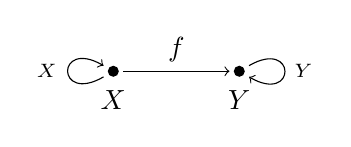
\begin{tikzpicture}
 \node (X) [label=below:{$X$}] at (-.8,0) {};
 \fill (X) circle[radius=2pt];
 \node (Y) [label=below:{$Y$}] at (.8,0) {};
 \fill (Y) circle[radius=2pt];
  \path (X) edge [loop left, out=-150,in=150,min distance=7mm, ->] node {$\id_X$} (X);
  \path (X) edge [->] node[above] {$f$} (Y);
  \path (Y) edge  [loop right, out=30,in=-30,min distance=7mm, ->] node {$\id_Y$} (Y);
\end{tikzpicture}
\]
\end{example}

\begin{example}[A group as a category] \label{exa:BG}
Let $G$ be a group. Consider the category $\rB G$ with one object
$\star$ (so $\ob\rB G = \{ \star\}$), and with $\Hom_{\rB G}(\star,\star) := G$, $\id_\star := 1 \in G$, and where composition is defined by multiplication in $G$. Note that axiom (C1) follows from the associativity of the group operation, and axiom (C2) from the axiom for the neutral element $1\in G$.
\end{example}

\begin{example}[Discrete category]\label{exa:discrete-cat}
If $S$ is a set, then $S$ defines a category $\cC$ with $\ob \cC := S$ and with
\[
	\Hom_\cC(x,y) := \begin{cases}  \{ \id \} & \text{if $x=y$} \\ \emptyset &\text{if $x\neq y$} \end{cases}
\]
for all $x,y\in S$.
\end{example}

\begin{example}[Pre-ordered set]\label{exa:pre-ordered}
A \emph{pre-ordered set} is a set $S$ equipped with a relation $\leq$ that is reflexive ($x\leq x$)  and transitive ($x\leq y$ and $y\leq z$ implies $x\leq z$). A pre-ordered set defines a category $\cC$ with $\ob \cC := S$ and with
\[
	\Hom_\cC(x,y) := \begin{cases}  \{  \star \} & \text{if $x\leq y$} \\ \emptyset &\text{if $x\not\leq y$} \end{cases}
\]
where $\{\star\}$ denotes any singleton. 
\end{example}

\begin{example}[The category of matrices] \label{exa:category-of-matrices}
Let $R$ be a ring. Then we can form a category $\cC$  with $\ob \cC :=\{ 0, 1, 2, \ldots \}$,  with
\[
	\Hom_\cC(n,m) := \Mat_{m,n}(R) := \{ \text{$m\times n$ matrices over $R$} \},
\]
and with composition being matrix multiplication
\[
	 \Mat_{m,\ell} \times \Mat_{\ell,k}  \to \Mat_{m,k}, (B,A) \mapsto BA.
\]
The identity element $\id_n\colon n \to n$ is the $n\times n$ identity matrix. Axiom (C1) corresponds to the associativity of matrix multiplication.
\end{example}

\begin{definition}\label{def:small-category}
A category is called \emph{locally small} if for every $X$ and $Y$ in $\ob \cC$ the class $\Hom_{\cC}(X,Y)$ is a set. It is called \emph{small} if moreover the class of objects $\ob \cC$ is itself a set.
\end{definition}

\begin{examples}
All the examples in sections~\ref{sec:big-examples} and \ref{sec:small-examples} are locally small. The examples in section~\ref{sec:small-examples} are in fact small. However, the examples in section~\ref{sec:big-examples} are not small, essentially because the class of all sets is not a set.
\end{examples}


Finally, we discuss two ways of constructing new categories out of old ones. The first is the opposite category, which is obtained by formally reversing all the arrows in a given category:
 
\begin{definition}\label{def:opposite-category}
The \emph{opposite} or \emph{dual} of a category $\cC$ is the category $\cC^\opp$ with $\ob \cC^\opp := \ob\cC$ and with
\[
	\Hom_{\cC^\opp}(X,Y) := \Hom_\cC(Y,X).
\]
Composition is done `the other way around': 
\[
	\Hom_{\cC^\opp}(Y,Z) \times \Hom_{\cC^\opp}(X,Y)   \to \Hom_{\cC^\opp}(X,Z),\,
	(g,f) \mapsto fg
\]
where $f\colon Y \to X$ and $g\colon Z\to Y$ and $fg\colon Z \to X$ are maps in $\cC$.
\end{definition}

\begin{definition}\label{def:product-category}
If $\cC$ and $\cD$ are categories, then the \emph{product category}
$\cC\times \cD$ is the category whose objects are pairs $(X,Y)$ with $X\in \ob \cC$ and $Y\in \ob \cD$, and whose morphisms are pairs of morphisms:
\[
	\Hom_{\cC\times \cD}((X,Y),(X',Y')) := \Hom_\cC(X,X') \times \Hom_\cD(Y,Y').
\]
\end{definition}

In general it makes no sense to ask if a morphism $f\colon X\to Y$ in a category $\cC$ is bijective, injective, or surjective. The objects $X$ and $Y$ are just elements of some class $\ob \cC$, and the morphism $f$ is just an element of some class $\Hom_\cC(X,Y)$.  It makes no sense to talk about elements of $X$ or $Y$. However, one can define what it means for $f$ to be an \emph{isomorphism}.


\begin{definition}Let $f\colon X\to Y$ be a morphism in a category $\cC$. We say that $f$ is an \emph{isomorphism} if there exists a morphism $g\colon Y \to X$ such that $fg=\id_Y$ and $gf=\id_X$.
\end{definition}

\begin{example}An isomorphism in $\Set$ is a bijection. An isomorphism in $\Grp$ is a group isomorphism. An isomorphism in $\Top$ is a homeomorphism (note that this is stronger than being a bijective continuous map!). An isomorphism in the category of matrices (Example \ref{exa:category-of-matrices}) is an invertible square matrix.
\end{example}

\begin{definition}We say that objects $X$ and $Y$ in a category are \emph{isomorphic} if there exists an isomorphism $f\colon X\to Y$.
\end{definition}

%\begin{definition}A morphism $f\colon X\to Y$ in a category $\cC$ is called a \emph{monomorphism} if
%for every object $T$ and for every pair of maps $g_1,g_2\colon T\to X$ with $fg_1=fg_2$ we have $g_1=g_2$.
%\end{definition}
%
%\begin{example}We claim that the monomorphisms in $\Set$ are precisely the injective functions. Indeed, if $f$ is injective, then clearly $fg_1 = fg_2$ implies $g_1=g_2$. Conversely, let $f\colon X\to Y$ be a monomorphism. Let $x_1,x_2\in X$ with $f(x_1)=f(x_2)$. Consider the one-element set $T=\{\star\}$ and the maps $g_i\colon T\to X,\, \star \mapsto x_i$. Then $fg_1=fg_2$, hence $g_1=g_2$, and therefore $x_1=x_2$.
%\end{example}
%
%\begin{example}By a similar argument one shows that the monomorphisms in $\Grp$ are precisely the injective group homomorphisms, see Exercise \ref{exc:monomorphisms-in-Grp}.
%\end{example}
%
%\begin{definition}A morphism $f\colon X\to Y$ in a category $\cC$ is called an \emph{epimorphism} if
%for every $T\in \ob \cC$ and for every pair of maps $g_1,g_2$ from $Y$ to $T$ with $g_1f=g_2f$ we have $g_1=g_2$.
%\end{definition}
%
%\begin{example}We claim that the epimorphisms in $\Set$ are precisely the surjective functions. Indeed, if $f$ is surjective and $g_1f=g_2f$, then certainly $g_1=g_2$. Conversely, let $f\colon X\to Y$ be an epimorphism. Assume that $f$ is not surjective, and pick an element $z\in Y$ not in the image of $f$. Consider the set $T:=\{0,1\}$ and maps 
%\[
%	g_1\colon Y \to T,\, y \mapsto 0
%\]
%and
%\[
%	g_2\colon Y \to T,\, y \mapsto \begin{cases} 0 & y \neq z \\ 1 & y = z \end{cases}
%\]
%Then $g_1f=g_2f$, but $g_1\neq g_2$, a contradiction.
%\end{example}


\section{Final and cofinal objects}

Some categories have special objects, called final and cofinal (also known as initial) objects. 

\begin{definition}
Let $\cC$ be a category. An object $X\in \ob \cC$ is called \emph{final} in $\cC$ if for every $Y\in \ob\cC$ there is a 
unique morphism $Y \to X$.
\end{definition}

\begin{definition}
Let $\cC$ be a category. An object $X\in \ob \cC$ is called \emph{cofinal} in $\cC$ if for every $Y\in \ob\cC$ there is a 
unique morphism $X\to Y$.
\end{definition}

\begin{examples}
In $\Top$ the empty space $\emptyset$ is a cofinal object, and a one-point space $\{\star\}$ is final. In ${}_R\Mod$ the zero module $0$ is both cofinal and final. In $\Ring$ the ring $\bZ$ is cofinal and the zero ring $0$ is final. In $\Grp$ the trivial group $\{1\}$ is both cofinal and final.
\end{examples}

\begin{proposition}\label{prop:final-object-uniquely-unique}
If it exists, a final object in a category $\cC$ is unique up to unique isomorphism.
\end{proposition}

\begin{proof}
Assume $X_1$ and $X_2$ are final. We need to show that there exists a unique isomorphism $f\colon X_1\to X_2$.

Since $X_2$ is final, there exists a map $f\colon X_1\to X_2$. Since $X_1$ is final, there exists a map $g\colon X_2\to X_1$. Consider the composite $fg\colon X_2 \to X_2$. Since $X_2$ is final, there is a unique map $X_2\to X_2$, so $fg=\id_{X_2}$. Similarly $gf=\id_{X_1}$. So we see that $f$ is an isomorphism $X_1\to X_2$.

Now assume that there are \emph{two} isomorphisms $f_1,f_2\colon X_1 \to X_2$. Then again, because $X_2$ is final, we must have $f_1=f_2$, which shows that $f$ is unique. 
\end{proof}

Like so many statements about categories, this proposition has a co-proposition:

\begin{proposition}
If it exists, a cofinal object in a category $\cC$ is unique up to unique isomorphism.
\end{proposition}

\begin{proof}Reverse the arrows in the proof of Proposition \ref{prop:final-object-uniquely-unique}. Alternatively, apply 
Proposition~\ref{prop:final-object-uniquely-unique} to the opposite category $\cC^\opp$.
\end{proof}

\newpage
\section*{Exercises}

\begin{exercise}[Automorphism group of an object]
Let $\cC$ be a (locally small) category and $X$ an object in $\cC$. Show that
\[
	\Aut_\cC(X) := \{ f\colon X\to X \mid \text{$f$ is an isomorphism} \}
\]
forms a group under composition.
\end{exercise}

\begin{exercise}
Let $\cC$ be a (locally small) category and $X$ and $Y$ objects in $\cC$. Assume that $X$ and $Y$ are isomorphic. Show that $\Aut_\cC(X)$ and $\Aut_\cC(Y)$ are isomorphic groups.
\end{exercise}

\begin{exercise}
Let $\cC$ be a category. Show that the relation `$X$ and $Y$ are isomorphic' forms an equivalence relation on $\ob \cC$.
\end{exercise}

\begin{exercise}
Let $f\colon X\to Y$ be a morphism in a category $\cC$. Show that if $f$ has both a left and a right inverse, then these must agree. In particular, $f$ has at most one two-sided inverse.
\end{exercise}

\begin{exercise}\label{exc:iso-category}
Let $\cC$ be a category. Define $\ob \cC^\times := \ob \cC$ and
\[
	\Hom_{\cC^\times}(X,Y) := \{ f \in \Hom_\cC(X,Y) \mid \text{$f$ is an isomorphism} \}.
\]
Show that $\cC^\times$ (with composition and identity maps inherited from $\cC$) is a category.
\end{exercise}

\begin{exercise}Verify that Examples~\ref{exa:one-arrow}  and~\ref{exa:discrete-cat} are special cases of Example~\ref{exa:pre-ordered}.
\end{exercise}

%\begin{exercise}\label{exc:monomorphisms-in-Grp}
%Show that the monomorphisms in $\Grp$ are precisely the injective group homomorphisms. (Hint: given $x\in G$ there is a group homomorphism $\bZ\to G$ which maps $1$ to $x$).
%\end{exercise}
%
%\begin{exercise}Let $R$ be a ring. Show that the monomorphisms in ${}_R\Mod$ are precisely the injective $R$-module homomorphisms.
%\end{exercise}
%
%\begin{exercise}Show that the epimorphisms in ${}_R\Mod$ are precisely the surjective  homomorphisms. (Hint: given $f\colon M\to N$ non-surjective, consider the module $\coker f$.)
%\end{exercise}

%
%\begin{exercise}
%Show that the map $\bZ\to\bQ$ in the category of rings is an epimorphism. Conclude that there exist morphisms that are both mono and epi, but not isomorphisms.
%\end{exercise}
%
%\begin{exercise}Let $\mathrm{\mathbf{Haus}}$ be the category of Hausdorff topological spaces and continuous maps. Let $f\colon X \to Y$ be a continuous map of Hausdorff spaces with dense image, show that $f$ is an epimorphism. (Hint: Let $g,h\colon Y \to T$ be continuous maps of topological spaces, with $T$ Hausdorff, show that $\{ x \in Y \mid g(x) = h(x) \}$ is closed). 
%\end{exercise}
%
%\begin{exercise}[$\star$] Show that the converse holds: if $f\colon X\to Y$ in $\mathrm{\mathbf{Haus}}$ is an epimorphism, then the image of $f$ is dense in $Y$.
%\end{exercise}
%
%
%\begin{exercise}[$\star\star$]Show that the epimorphisms in $\Grp$ are precisely the surjective group homomorphisms.
%\end{exercise}
%
%\begin{exercise}
%What are the isomorphisms, monomorphisms and epimorphisms in the matrix category over a field $K$? (See Example \ref{exa:category-of-matrices}).
%\end{exercise}

\begin{exercise}Show that the category of fields has neither final nor cofinal object. Show that the category of fields of a given fixed characteristic does have a cofinal object.
\end{exercise}

%\begin{exercise}[Split monomorphisms]\label{exc:split-mono}
%Let $f\colon X\to Y$ be a morphism in $\cC$. Assume that there exists a morphism $g\colon Y\to X$ with $gf=\id_X$. Show that $f$ is a monomorphism. Such $f$ is called a \emph{split monomorphism}. Give an example of a monomorphism that is not a split monomorphism.
%\end{exercise}
%
%\begin{exercise}[Split epimorphisms]\label{exc:split-epi}
%Let $f\colon X\to Y$ be a morphism in $\cC$. Assume that there exists a morphism $g\colon Y\to X$ with $fg=\id_Y$. Show that $f$ is an epimorphism. Such $f$ is called a \emph{split epimorphism}. Give an example of an epimorphism that is not a split epimorphism.
%\end{exercise}


\begin{exercise}[The category of $G$-sets] Let $G$ be a group. A $G$-set is a set $S$ together with a left action of $G$ on $S$, that is, a map $G\times S \to S,\, (g,s)\mapsto gs$ satisfying $1s=s$ and $g(hs)=(gh)s$ for all $g,h \in G$ and $s\in S$. A morphism of $G$-sets is a map $f\colon S\to T$ satisfying $f(gs)=gf(s)$ for every $s\in S$ and $g\in G$. The category of $G$-sets is denoted $_{G}\Set$. 

What are the final and cofinal objects of $_{G}\Set$? 
\end{exercise}

\begin{exercise}
Let $\cC$ be a category and $X$ and $Y$ objectsin $\cC$. Assume that $X$ is final, and that $X$ and $Y$ are isomorphic. Show that $Y$ is also final.
\end{exercise}


\begin{exercise}[Homotopy category]
Let $\hTop$ be the \emph{homotopy category} of topological spaces. Its objects are 
topological spaces, and its morphisms are \emph{homotopy classes} of continuous maps:
\[
	\Hom_{\hTop}(X,Y) := \{ f\colon X\to Y \mid \text{$f$ continuous}\}/\sim
\]
(Note that composition is compatible with homotopy, so that composition in $\hTop$ is well-defined). Show that two topological spaces $X$ and $Y$ are homotopy-equivalent if and only if $X$ and $Y$ are isomorphic in the category $\hTop$. 
\end{exercise}

\begin{exercise}\label{exc:yoneda-isomorphism-test}
Let $f\colon X\to Y$ be a morphism in $\cC$. Show that $f$ is an isomorphism if and only if for all objects $T$ in $\cC$ the map
\[
	\Hom_\cC(T,X) \to \Hom_\cC(T,Y),\, h \mapsto fh
\]
is a bijection. (Hint, for the hard direction: use $T=Y$ to find a $g\colon Y\to X$ with $fg=\id_Y$, and use $T=X$ to deduce that $gf=\id_X$.)
\end{exercise}

\begin{exercise}Formulate and prove the co-Exercise of Exercise~\ref{exc:yoneda-isomorphism-test}.
\end{exercise}

%%%%%%%%%%%%%%%%%%%%%%
% FUNCTORS AND EQUIVALENCES
%%%%%%%%%%%%%%%%%%%%%%%

